\documentclass[smallextended]{svjour3}
\usepackage[]{graphicx}\usepackage[]{xcolor}
% maxwidth is the original width if it is less than linewidth
% otherwise use linewidth (to make sure the graphics do not exceed the margin)
\makeatletter
\def\maxwidth{ %
  \ifdim\Gin@nat@width>\linewidth
    \linewidth
  \else
    \Gin@nat@width
  \fi
}
\makeatother

\definecolor{fgcolor}{rgb}{0.345, 0.345, 0.345}
\newcommand{\hlnum}[1]{\textcolor[rgb]{0.686,0.059,0.569}{#1}}%
\newcommand{\hlstr}[1]{\textcolor[rgb]{0.192,0.494,0.8}{#1}}%
\newcommand{\hlcom}[1]{\textcolor[rgb]{0.678,0.584,0.686}{\textit{#1}}}%
\newcommand{\hlopt}[1]{\textcolor[rgb]{0,0,0}{#1}}%
\newcommand{\hlstd}[1]{\textcolor[rgb]{0.345,0.345,0.345}{#1}}%
\newcommand{\hlkwa}[1]{\textcolor[rgb]{0.161,0.373,0.58}{\textbf{#1}}}%
\newcommand{\hlkwb}[1]{\textcolor[rgb]{0.69,0.353,0.396}{#1}}%
\newcommand{\hlkwc}[1]{\textcolor[rgb]{0.333,0.667,0.333}{#1}}%
\newcommand{\hlkwd}[1]{\textcolor[rgb]{0.737,0.353,0.396}{\textbf{#1}}}%
\let\hlipl\hlkwb

\usepackage{framed}
\makeatletter
\newenvironment{kframe}{%
 \def\at@end@of@kframe{}%
 \ifinner\ifhmode%
  \def\at@end@of@kframe{\end{minipage}}%
  \begin{minipage}{\columnwidth}%
 \fi\fi%
 \def\FrameCommand##1{\hskip\@totalleftmargin \hskip-\fboxsep
 \colorbox{shadecolor}{##1}\hskip-\fboxsep
     % There is no \\@totalrightmargin, so:
     \hskip-\linewidth \hskip-\@totalleftmargin \hskip\columnwidth}%
 \MakeFramed {\advance\hsize-\width
   \@totalleftmargin\z@ \linewidth\hsize
   \@setminipage}}%
 {\par\unskip\endMakeFramed%
 \at@end@of@kframe}
\makeatother

\definecolor{shadecolor}{rgb}{.97, .97, .97}
\definecolor{messagecolor}{rgb}{0, 0, 0}
\definecolor{warningcolor}{rgb}{1, 0, 1}
\definecolor{errorcolor}{rgb}{1, 0, 0}
\newenvironment{knitrout}{}{} % an empty environment to be redefined in TeX

\usepackage{alltt}
\newcommand{\SweaveOpts}[1]{}  % do not interfere with LaTeX
\newcommand{\SweaveInput}[1]{} % because they are not real TeX commands
\newcommand{\Sexpr}[1]{}       % will only be parsed by R

    
\smartqed  % flush right qed marks, e.g. at end of proof

\usepackage[colorlinks=true,linkcolor={blue},citecolor={blue},urlcolor={blue}]{hyperref}
%\usepackage{caption}
% Add longtable and ctable packages
\usepackage{longtable,ctable}
\usepackage{amsmath}
\usepackage{amssymb}
\usepackage{amsfonts}
\usepackage{multirow}
%\usepackage{amsthm}
\usepackage{graphicx}

\usepackage{booktabs}
%\usepackage{bookmark}

%\usepackage{caption}
%\usepackage{capt-of}

\usepackage{amsmath}
\usepackage{graphicx}
\usepackage{mathptmx}
\usepackage{natbib}

\usepackage{setspace}

%\usepackage{tikz-feynman}
%\usepackage{tikz} 
%\usetikzlibrary{positioning}
\usepackage[utf8]{inputenc}
\usepackage{pgf}


\usepackage{algorithm}
\usepackage{algpseudocode}
\usepackage{enumerate}

\usepackage{threeparttable}

\raggedbottom

\newcommand{\R}{R}
\newcommand{\gbsg}{gbsg}

%\def\FsNg{\hbox{FS}(M_{g})}

\def\FsNg{\hbox{FS-M}}

\def\hhat{\hat\theta(\hat{H})}
\def\hchat{\hat\theta(\hat{H}^{c})}
\def\hknow{\hat\theta(H)}
\def\hcknow{\hat\theta(H^{c})}
\def\hplim{\theta^{\dagger}(H)}
\def\hcplim{\theta^{\dagger}(H^{c})}

\def\sumin{\sum_{i=1}^n}
\def\nsumin{n^{-1}\sum_{i=1}^n}

\def\ns{n_{0}+n_{1}}
\def\na{n_{0}}
\def\nb{n_{1}}

\newcommand{\indep}{\perp \!\!\! \perp}

\textheight=9.25in \textwidth=6.0in 
\topmargin=0in
\evensidemargin=0in \oddsidemargin=0in



\begin{document}





\begin{knitrout}
\definecolor{shadecolor}{rgb}{0.969, 0.969, 0.969}\color{fgcolor}\begin{kframe}
\begin{alltt}
\hlkwd{rm}\hlstd{(}\hlkwc{list} \hlstd{=} \hlkwd{ls}\hlstd{())}

\hlcom{# Local github}
\hlstd{codepath} \hlkwb{<-} \hlkwd{c}\hlstd{(}\hlstr{"/media/larryleon/My Projects/GitHub/Forest-Search/R/"}\hlstd{)}
\hlkwd{source}\hlstd{(}\hlkwd{paste0}\hlstd{(codepath,} \hlstr{"source_forestsearch_v0.R"}\hlstd{))}
\hlkwd{source_fs_functions}\hlstd{(}\hlkwc{file_loc} \hlstd{= codepath)}

\hlkwd{library}\hlstd{(kableExtra)}
\hlkwd{library}\hlstd{(knitr)}
\hlkwd{library}\hlstd{(ggplot2)}
\hlkwd{library}\hlstd{(gridExtra)}
\hlkwd{library}\hlstd{(cubature)}
\hlkwd{library}\hlstd{(aVirtualTwins)}
\hlkwd{library}\hlstd{(randomForest)}
\hlkwd{library}\hlstd{(survival)}
\hlkwd{library}\hlstd{(survminer)}
\hlkwd{library}\hlstd{(grf)}
\hlkwd{library}\hlstd{(policytree)}
\hlkwd{library}\hlstd{(data.table)}
\hlkwd{library}\hlstd{(plyr)}
\hlkwd{library}\hlstd{(dplyr)}
\hlkwd{library}\hlstd{(glmnet)}
\hlkwd{library}\hlstd{(corrplot)}
\end{alltt}
\end{kframe}
\end{knitrout}




\begin{knitrout}
\definecolor{shadecolor}{rgb}{0.969, 0.969, 0.969}\color{fgcolor}\begin{kframe}
\begin{alltt}
\hlstd{maxFollow} \hlkwb{<-} \hlnum{84}
\hlstd{cens.type} \hlkwb{<-} \hlstr{"weibull"}

\hlcom{# m1 -censoring adjustment}
\hlstd{muC.adj} \hlkwb{<-} \hlkwd{log}\hlstd{(}\hlnum{1.5}\hlstd{)}
\hlstd{k.z3} \hlkwb{<-} \hlnum{1}
\hlstd{k.treat} \hlkwb{<-} \hlnum{0.9}

\hlstd{z1_frac} \hlkwb{<-} \hlnum{0.25}  \hlcom{# Default model index 'm1' (The 1st quartile of z1=er)}
\hlstd{pH_super} \hlkwb{<-} \hlnum{0.125}  \hlcom{# non-NULL re-defines z1_frac}

\hlkwa{if} \hlstd{(}\hlkwd{is.null}\hlstd{(pH_super)) \{}
    \hlcom{# pH_check<-with(gbsg,mean(pgr<=quantile(pgr,c(z3_frac),1,0) &}
    \hlcom{# er<=quantile(er,z1_frac)))}
    \hlstd{pH_check} \hlkwb{<-} \hlkwd{with}\hlstd{(gbsg,} \hlkwd{mean}\hlstd{(meno} \hlopt{==} \hlnum{0} \hlopt{&} \hlstd{er} \hlopt{<=} \hlkwd{quantile}\hlstd{(er, z1_frac)))}
    \hlkwd{cat}\hlstd{(}\hlstr{"Underlying pH_super"}\hlstd{,} \hlkwd{c}\hlstd{(pH_check),} \hlstr{"\textbackslash{}n"}\hlstd{)}
\hlstd{\}}
\hlcom{# pH_super specified If pH_super then override z1_frac and find z1_frac to}
\hlcom{# yield pH_super}

\hlkwa{if} \hlstd{(}\hlopt{!}\hlkwd{is.null}\hlstd{(pH_super)) \{}
    \hlcom{# Approximate Z1 quantile to yield pH proportion}
    \hlstd{z1_q} \hlkwb{<-} \hlkwd{uniroot}\hlstd{(propH.obj4,} \hlkwd{c}\hlstd{(}\hlnum{0}\hlstd{,} \hlnum{1}\hlstd{),} \hlkwc{tol} \hlstd{=} \hlnum{1e-04}\hlstd{,} \hlkwc{pH.target} \hlstd{= pH_super)}\hlopt{$}\hlstd{root}
    \hlcom{# pH_check<-with(gbsg,mean(pgr<=quantile(pgr,c(z3_frac),1,0) &}
    \hlcom{# er<=quantile(er,z1_q)))}
    \hlstd{pH_check} \hlkwb{<-} \hlkwd{with}\hlstd{(gbsg,} \hlkwd{mean}\hlstd{(meno} \hlopt{==} \hlnum{0} \hlopt{&} \hlstd{er} \hlopt{<=} \hlkwd{quantile}\hlstd{(er, z1_q)))}
    \hlkwd{cat}\hlstd{(}\hlstr{"pH"}\hlstd{,} \hlkwd{c}\hlstd{(pH_check),} \hlstr{"\textbackslash{}n"}\hlstd{)}
    \hlstd{rel_error} \hlkwb{<-} \hlstd{(pH_super} \hlopt{-} \hlstd{pH_check)}\hlopt{/}\hlstd{pH_super}
    \hlkwa{if} \hlstd{(}\hlkwd{abs}\hlstd{(rel_error)} \hlopt{>=} \hlnum{0.1}\hlstd{)}
        \hlkwd{stop}\hlstd{(}\hlstr{"pH_super approximation relative error exceeds 10%"}\hlstd{)}
    \hlstd{z1_frac} \hlkwb{<-} \hlstd{z1_q}
    \hlkwd{cat}\hlstd{(}\hlstr{"Underlying pH_super"}\hlstd{,} \hlkwd{c}\hlstd{(pH_check),} \hlstr{"\textbackslash{}n"}\hlstd{)}
\hlstd{\}}
\end{alltt}
\begin{verbatim}
## pH 0.122449 
## Underlying pH_super 0.122449
\end{verbatim}
\begin{alltt}
\hlcom{# Bootstrap on log(hr) scale converted to HR (est.loghr=TRUE & est.scale='hr')}
\hlstd{t.start.all} \hlkwb{<-} \hlkwd{proc.time}\hlstd{()[}\hlnum{3}\hlstd{]}
\end{alltt}
\end{kframe}
\end{knitrout}


\begin{knitrout}
\definecolor{shadecolor}{rgb}{0.969, 0.969, 0.969}\color{fgcolor}\begin{kframe}
\begin{alltt}
\hlcom{######################### Forest search criteria}
\hlstd{hr.threshold} \hlkwb{<-} \hlnum{1.25}  \hlcom{# Initital candidates }
\hlstd{hr.consistency} \hlkwb{<-} \hlnum{1}  \hlcom{# Candidates for many splits}
\hlstd{pconsistency.threshold} \hlkwb{<-} \hlnum{0.9}
\hlstd{stop.threshold} \hlkwb{<-} \hlnum{0.95}
\hlstd{maxk} \hlkwb{<-} \hlnum{2}
\hlstd{nmin.fs} \hlkwb{<-} \hlnum{60}
\hlstd{pstop_futile} \hlkwb{<-} \hlnum{0.5}
\hlcom{# Limit timing for forestsearch}
\hlstd{max.minutes} \hlkwb{<-} \hlnum{3}
\hlstd{m1.threshold} \hlkwb{<-} \hlnum{Inf}  \hlcom{# Turning this off (Default)}
\hlcom{# pconsistency.threshold<-0.70 # Minimum threshold (will choose max among}
\hlcom{# subgroups satisfying)}
\hlstd{fs.splits} \hlkwb{<-} \hlnum{400}  \hlcom{# How many times to split for consistency}
\hlcom{# vi is % factor is selected in cross-validation --> higher more important}
\hlstd{vi.grf.min} \hlkwb{<-} \hlnum{0.2}
\hlcom{# Null, turns off grf screening}
\hlstd{d.min} \hlkwb{<-} \hlnum{10}  \hlcom{# Min number of events for both arms (d0.min=d1.min=d.min)}
\hlcom{# default=5 Virtual twins analysis Counter-factual difference (C-E) >=}
\hlcom{# vt.threshold Large values in favor of C (control)}
\hlstd{vt.threshold} \hlkwb{<-} \hlnum{0.225}  \hlcom{# For VT delta}
\hlstd{treat.threshold} \hlkwb{<-} \hlnum{0}

\hlstd{maxdepth} \hlkwb{<-} \hlnum{2}
\hlstd{n.min} \hlkwb{<-} \hlnum{60}
\hlstd{ntree} \hlkwb{<-} \hlnum{1000}
\hlcom{# GRF criteria}
\hlstd{dmin.grf} \hlkwb{<-} \hlnum{12}  \hlcom{# For GRF delta}
\hlcom{# Note: For CRT this represents dmin.grf/2 RMS for control (-dmin.grf/2 for}
\hlcom{# treatment)}
\hlstd{frac.tau} \hlkwb{<-} \hlnum{0.6}

\hlstd{outcome.name} \hlkwb{<-} \hlkwd{c}\hlstd{(}\hlstr{"y.sim"}\hlstd{)}
\hlstd{event.name} \hlkwb{<-} \hlkwd{c}\hlstd{(}\hlstr{"event.sim"}\hlstd{)}
\hlstd{id.name} \hlkwb{<-} \hlkwd{c}\hlstd{(}\hlstr{"id"}\hlstd{)}
\hlstd{treat.name} \hlkwb{<-} \hlkwd{c}\hlstd{(}\hlstr{"treat"}\hlstd{)}

\hlstd{cox.formula.sim} \hlkwb{<-} \hlkwd{as.formula}\hlstd{(}\hlkwd{paste}\hlstd{(}\hlstr{"Surv(y.sim,event.sim)~treat"}\hlstd{))}
\hlstd{cox.formula.adj.sim} \hlkwb{<-} \hlkwd{as.formula}\hlstd{(}\hlkwd{paste}\hlstd{(}\hlstr{"Surv(y.sim,event.sim)~treat+v1+v2+v3+v4+v5"}\hlstd{))}
\end{alltt}
\end{kframe}
\end{knitrout}



\begin{knitrout}
\definecolor{shadecolor}{rgb}{0.969, 0.969, 0.969}\color{fgcolor}\begin{kframe}
\begin{alltt}
\hlstd{mod.harm} \hlkwb{<-} \hlstr{"alt"}
\hlstd{hrH.target} \hlkwb{<-} \hlnum{2.5}
\hlcom{# out.loc = NULL turns off file creation}
\hlstd{N} \hlkwb{<-} \hlnum{700}
\hlstd{this.dgm} \hlkwb{<-} \hlkwd{get.dgm4}\hlstd{(}\hlkwc{mod.harm} \hlstd{= mod.harm,} \hlkwc{N} \hlstd{= N,} \hlkwc{k.treat} \hlstd{= k.treat,} \hlkwc{hrH.target} \hlstd{= hrH.target,}
    \hlkwc{cens.type} \hlstd{= cens.type,} \hlkwc{out.loc} \hlstd{=} \hlkwa{NULL}\hlstd{,} \hlkwc{details} \hlstd{=} \hlnum{TRUE}\hlstd{,} \hlkwc{parms_torand} \hlstd{=} \hlnum{FALSE}\hlstd{)}
\end{alltt}
\end{kframe}
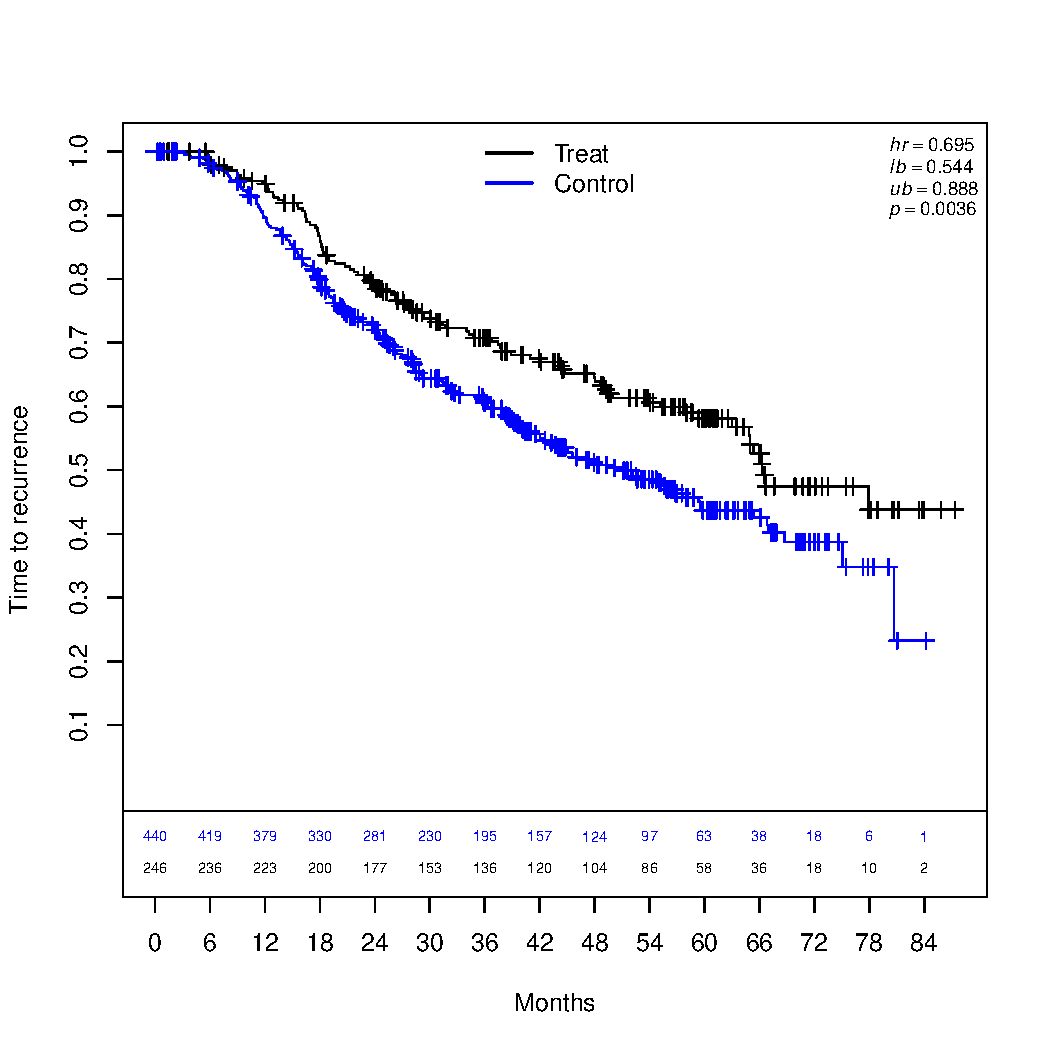
\includegraphics[width=\maxwidth]{figure/r_DGMsetup-1} 
\begin{kframe}\begin{verbatim}
## Super-population empirical harm and non-harm hazard ratios= 2.499996 0.6466405 
## Causal HR (empirical ITT)= 0.7125876
\end{verbatim}
\end{kframe}
\end{knitrout}

\begin{knitrout}
\definecolor{shadecolor}{rgb}{0.969, 0.969, 0.969}\color{fgcolor}\begin{kframe}
\begin{alltt}
\hlstd{n_add_noise} \hlkwb{<-} \hlnum{3}

\hlcom{# sim=69 sim=71}

\hlstd{sim} \hlkwb{<-} \hlnum{72}

\hlstd{dgm} \hlkwb{<-} \hlstd{this.dgm}\hlopt{$}\hlstd{dgm}

\hlstd{x} \hlkwb{<-} \hlkwd{sim_aftm4_gbsg}\hlstd{(}\hlkwc{dgm} \hlstd{= dgm,} \hlkwc{n} \hlstd{= N,} \hlkwc{maxFollow} \hlstd{= maxFollow,} \hlkwc{muC.adj} \hlstd{= muC.adj,} \hlkwc{simid} \hlstd{= sim)}

\hlstd{kmfit} \hlkwb{<-} \hlkwd{survfit}\hlstd{(}\hlkwd{Surv}\hlstd{(y.sim, event)} \hlopt{~} \hlstd{treat,} \hlkwc{data} \hlstd{= x)}

\hlkwd{ggsurvplot}\hlstd{(kmfit,} \hlkwc{data} \hlstd{= x,} \hlkwc{main} \hlstd{=} \hlstr{"K-M curves for simulated data"}\hlstd{,} \hlkwc{legend} \hlstd{=} \hlstr{"top"}\hlstd{,}
    \hlkwc{legend.title} \hlstd{=} \hlstr{"Treatment"}\hlstd{,} \hlkwc{legend.labs} \hlstd{=} \hlkwd{c}\hlstd{(}\hlstr{"Control"}\hlstd{,} \hlstr{"Experimental"}\hlstd{),} \hlkwc{palette} \hlstd{=} \hlstr{"grey"}\hlstd{,}
    \hlkwc{risk.table} \hlstd{=} \hlnum{TRUE}\hlstd{,} \hlkwc{risk.table.col} \hlstd{=} \hlstr{"strata"}\hlstd{)}
\end{alltt}
\end{kframe}
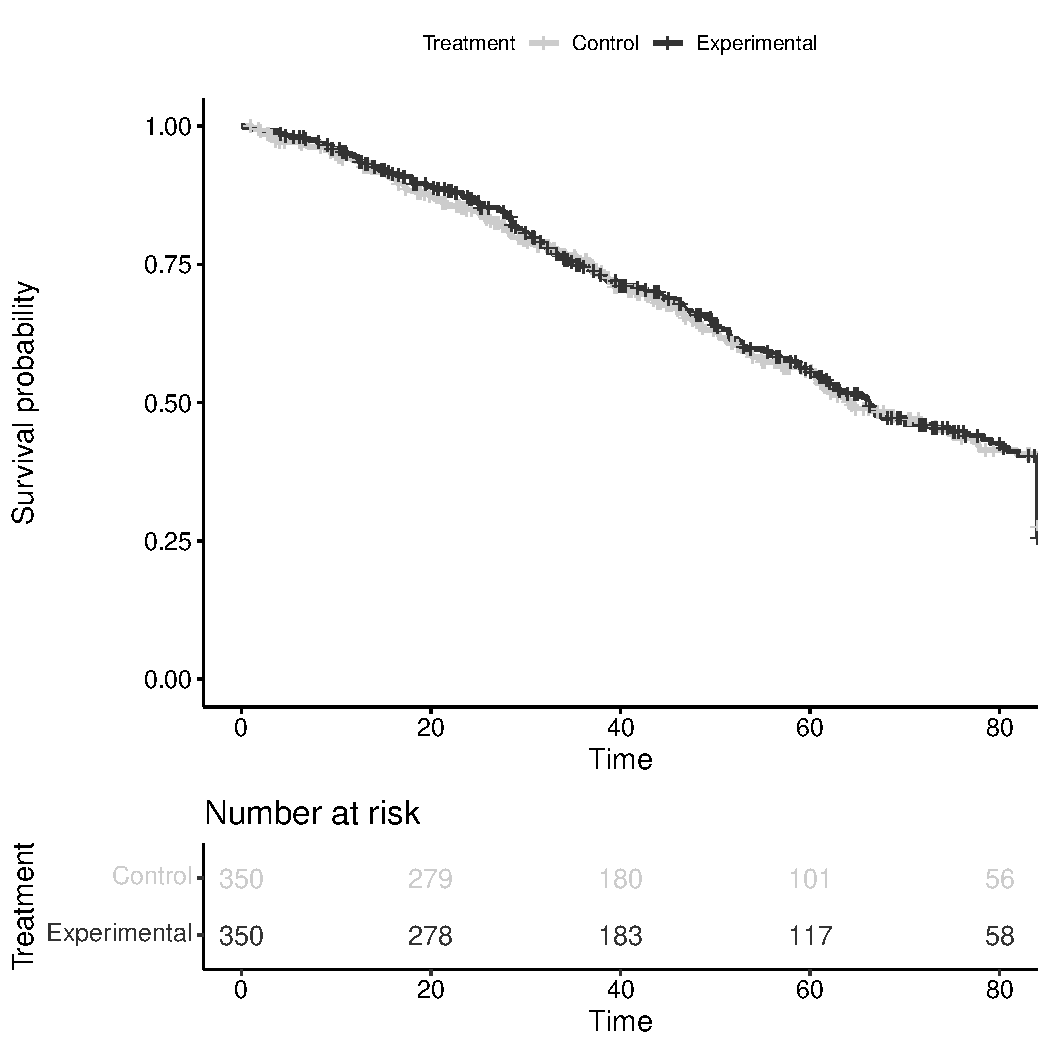
\includegraphics[width=\maxwidth]{figure/r_Simdata-1} 
\end{knitrout}


\begin{knitrout}
\definecolor{shadecolor}{rgb}{0.969, 0.969, 0.969}\color{fgcolor}\begin{kframe}
\begin{alltt}
\hlkwa{if} \hlstd{(n_add_noise} \hlopt{==} \hlnum{0}\hlstd{) \{}
    \hlstd{confounders.name} \hlkwb{<-} \hlkwd{c}\hlstd{(}\hlstr{"z1"}\hlstd{,} \hlstr{"z2"}\hlstd{,} \hlstr{"z3"}\hlstd{,} \hlstr{"z4"}\hlstd{,} \hlstr{"z5"}\hlstd{,} \hlstr{"size"}\hlstd{,} \hlstr{"grade"}\hlstd{)}
\hlstd{\}}

\hlkwa{if} \hlstd{(n_add_noise} \hlopt{==} \hlnum{5}\hlstd{) \{}
    \hlkwd{set.seed}\hlstd{(}\hlnum{8316951} \hlopt{+} \hlnum{1000} \hlopt{*} \hlstd{sim)}
    \hlcom{# Add 5 noise}
    \hlstd{x}\hlopt{$}\hlstd{noise1} \hlkwb{<-} \hlkwd{rnorm}\hlstd{(N)}
    \hlstd{x}\hlopt{$}\hlstd{noise2} \hlkwb{<-} \hlkwd{rnorm}\hlstd{(N)}
    \hlstd{x}\hlopt{$}\hlstd{noise3} \hlkwb{<-} \hlkwd{rnorm}\hlstd{(N)}
    \hlstd{x}\hlopt{$}\hlstd{noise4} \hlkwb{<-} \hlkwd{rnorm}\hlstd{(N)}
    \hlstd{x}\hlopt{$}\hlstd{noise5} \hlkwb{<-} \hlkwd{rnorm}\hlstd{(N)}
    \hlstd{confounders.name} \hlkwb{<-} \hlkwd{c}\hlstd{(}\hlstr{"z1"}\hlstd{,} \hlstr{"z2"}\hlstd{,} \hlstr{"z3"}\hlstd{,} \hlstr{"z4"}\hlstd{,} \hlstr{"z5"}\hlstd{,} \hlstr{"size"}\hlstd{,} \hlstr{"grade"}\hlstd{,} \hlstr{"noise1"}\hlstd{,}
        \hlstr{"noise2"}\hlstd{,} \hlstr{"noise3"}\hlstd{,} \hlstr{"noise4"}\hlstd{,} \hlstr{"noise5"}\hlstd{)}
\hlstd{\}}

\hlkwa{if} \hlstd{(n_add_noise} \hlopt{==} \hlnum{3}\hlstd{) \{}
    \hlkwd{set.seed}\hlstd{(}\hlnum{8316951} \hlopt{+} \hlnum{1000} \hlopt{*} \hlstd{sim)}
    \hlcom{# Add 3 noise}
    \hlstd{x}\hlopt{$}\hlstd{noise1} \hlkwb{<-} \hlkwd{rnorm}\hlstd{(N,} \hlkwc{sd} \hlstd{=} \hlnum{1}\hlstd{)}
    \hlstd{x}\hlopt{$}\hlstd{noise2} \hlkwb{<-} \hlkwd{rnorm}\hlstd{(N,} \hlkwc{sd} \hlstd{=} \hlnum{1}\hlstd{)}
    \hlstd{x}\hlopt{$}\hlstd{noise3} \hlkwb{<-} \hlkwd{rnorm}\hlstd{(N,} \hlkwc{sd} \hlstd{=} \hlnum{1}\hlstd{)}
    \hlstd{confounders.name} \hlkwb{<-} \hlkwd{c}\hlstd{(}\hlstr{"z1"}\hlstd{,} \hlstr{"z2"}\hlstd{,} \hlstr{"z3"}\hlstd{,} \hlstr{"z4"}\hlstd{,} \hlstr{"z5"}\hlstd{,} \hlstr{"size"}\hlstd{,} \hlstr{"grade"}\hlstd{,} \hlstr{"noise1"}\hlstd{,}
        \hlstr{"noise2"}\hlstd{,} \hlstr{"noise3"}\hlstd{)}
\hlstd{\}}

\hlcom{# More challenging which_replace <- which(confounders.name=='z1')}
\hlcom{# confounders.name[which_replace] <- 'er'}

\hlstd{cox.formula.check} \hlkwb{<-} \hlkwd{as.formula}\hlstd{(}\hlkwd{paste}\hlstd{(}\hlstr{"Surv(y.sim,event.sim)~treat+v1+v2+v3+v4+v5+size+grade+noise1+noise2+noise3"}\hlstd{))}
\hlkwd{coxph}\hlstd{(cox.formula.check,} \hlkwc{data} \hlstd{= x)}
\end{alltt}
\begin{verbatim}
## Call:
## coxph(formula = cox.formula.check, data = x)
## 
##             coef exp(coef)  se(coef)      z        p
## treat  -0.190082  0.826891  0.103686 -1.833 0.066765
## v11     0.387179  1.472819  0.126681  3.056 0.002241
## v21    -0.433922  0.647962  0.165536 -2.621 0.008759
## v31     0.597880  1.818260  0.169221  3.533 0.000411
## v41     1.037769  2.822913  0.126076  8.231  < 2e-16
## v51    -0.979521  0.375491  0.111687 -8.770  < 2e-16
## size   -0.003174  0.996831  0.003292 -0.964 0.334838
## grade  -0.118861  0.887931  0.096446 -1.232 0.217794
## noise1 -0.027040  0.973322  0.050086 -0.540 0.589285
## noise2  0.071227  1.073825  0.054128  1.316 0.188202
## noise3 -0.029600  0.970834  0.054628 -0.542 0.587927
## 
## Likelihood ratio test=214.1  on 11 df, p=< 2.2e-16
## n= 700, number of events= 386
\end{verbatim}
\begin{alltt}
\hlstd{Zm} \hlkwb{<-} \hlkwd{cor}\hlstd{(}\hlkwd{as.matrix}\hlstd{(x[,} \hlkwd{c}\hlstd{(confounders.name)]))}
\hlkwd{corrplot}\hlstd{(Zm)}
\end{alltt}
\end{kframe}
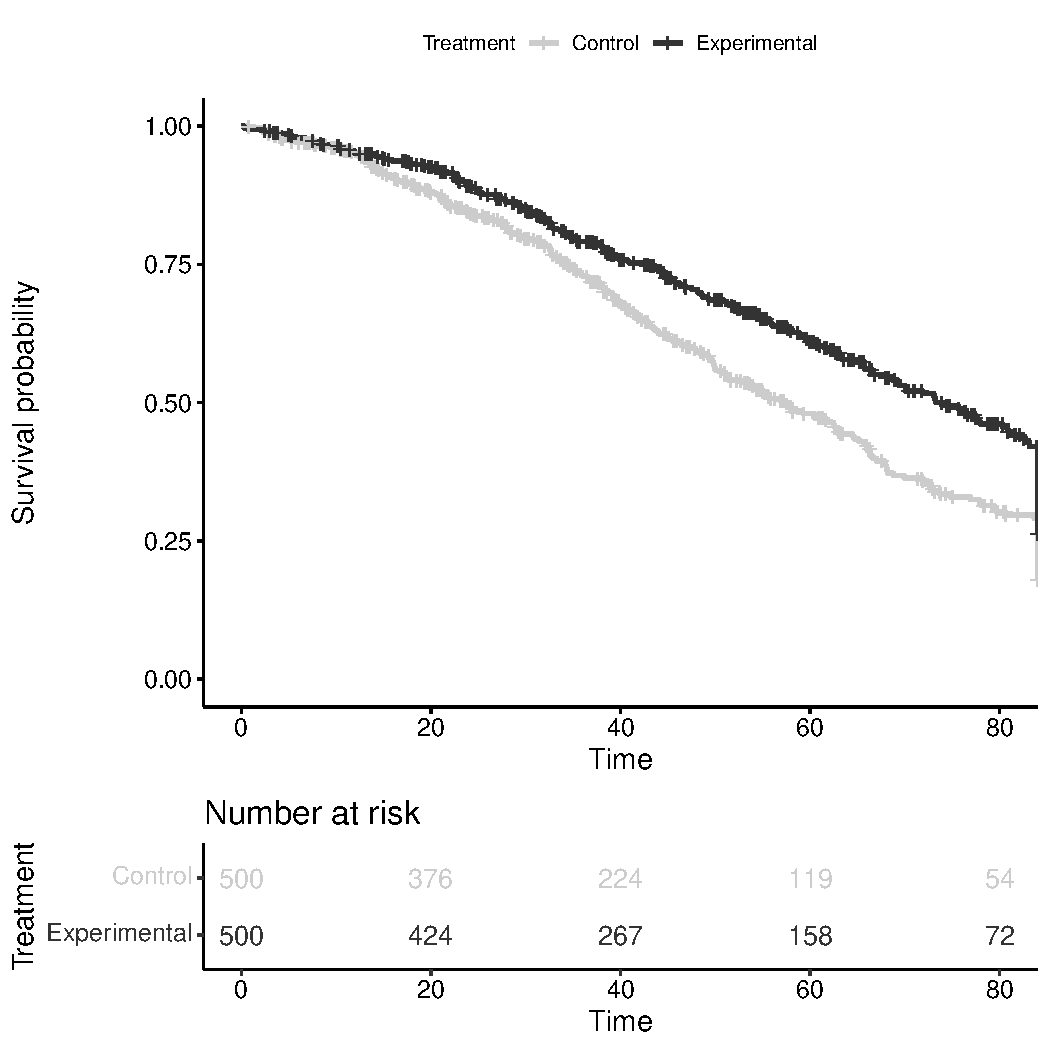
\includegraphics[width=\maxwidth]{figure/r_FSanalysis-1} 
\begin{kframe}\begin{alltt}
\hlcom{# Options Allconfounders.name is list of confounders within analysis dataset}
\hlcom{# (1) use_lasso=TRUE & use_grf=FALSE Lasso used to possibly reduce dimension}
\hlcom{# Any continuous factors are cut at medians (2) use_lasso=TRUE & use_grf=TRUE}
\hlcom{# Lasso used to reduce dimension Continuous covariates are cut at medians}
\hlcom{# However, if GRF selects a covariate cut then only that cut is used: For}
\hlcom{# example if 'age <= median(ag)' is called for per Lasso but GRF includes 'age}
\hlcom{# <= 54', then only the latter is used (3) use_grf_only = TRUE (overrides}
\hlcom{# use_lasso and use_grf) Only factors selected via GRF are used (4) use_lasso =}
\hlcom{# F & use_grf =T Median cuts (unless selected via GRF) as in (2) However no}
\hlcom{# possible dimension reduction via lasso All categorical factors included}

\hlstd{use_lasso} \hlkwb{<-} \hlnum{TRUE}
\hlstd{use_grf} \hlkwb{<-} \hlnum{FALSE}
\hlstd{use_grf_only} \hlkwb{<-} \hlnum{FALSE}

\hlstd{fs.est} \hlkwb{<-} \hlkwd{forestsearch}\hlstd{(}\hlkwc{df.analysis} \hlstd{= x,} \hlkwc{Allconfounders.name} \hlstd{= confounders.name,} \hlkwc{details} \hlstd{=} \hlnum{TRUE}\hlstd{,}
    \hlkwc{use_lasso} \hlstd{= use_lasso,} \hlkwc{use_grf} \hlstd{= use_grf,} \hlkwc{use_grf_only} \hlstd{= use_grf_only,} \hlkwc{dmin.grf} \hlstd{=} \hlnum{12}\hlstd{,}
    \hlkwc{frac.tau} \hlstd{=} \hlnum{0.6}\hlstd{,} \hlkwc{conf_force} \hlstd{=} \hlkwa{NULL}\hlstd{,} \hlkwc{outcome.name} \hlstd{= outcome.name,} \hlkwc{treat.name} \hlstd{= treat.name,}
    \hlkwc{event.name} \hlstd{= event.name,} \hlkwc{id.name} \hlstd{= id.name,} \hlkwc{n.min} \hlstd{= nmin.fs,} \hlkwc{hr.threshold} \hlstd{= hr.threshold,}
    \hlkwc{hr.consistency} \hlstd{= hr.consistency,} \hlkwc{fs.splits} \hlstd{= fs.splits,} \hlkwc{d0.min} \hlstd{= d.min,} \hlkwc{d1.min} \hlstd{= d.min,}
    \hlkwc{pstop_futile} \hlstd{= pstop_futile,} \hlkwc{pconsistency.threshold} \hlstd{= pconsistency.threshold,}
    \hlkwc{stop.threshold} \hlstd{= stop.threshold,} \hlkwc{max.minutes} \hlstd{= max.minutes,} \hlkwc{maxk} \hlstd{= maxk,} \hlkwc{by.risk} \hlstd{=} \hlnum{12}\hlstd{,}
    \hlkwc{plot.sg} \hlstd{=} \hlnum{TRUE}\hlstd{,} \hlkwc{vi.grf.min} \hlstd{= vi.grf.min)}
\end{alltt}
\begin{verbatim}
## # of continuous/categorical characteristics 4 6 
## Continuous characteristics: size noise1 noise2 noise3 
## Categorical characteristics: z1 z2 z3 z4 z5 grade 
## 10 x 2 sparse Matrix of class "dgCMatrix"
##                  s0          s0
## z1      0.387935497 0.384231095
## z2     -0.388657310 0.384946015
## z3      0.562310317 0.556940807
## z4      1.009641078 1.000000000
## z5     -0.971332113 0.962056848
## size   -0.002845356 0.002818186
## grade  -0.105237827 0.104232910
## noise1 -0.032215335 0.031907711
## noise2  0.063340373 0.062735534
## noise3 -0.031218814 0.030920705
## Cox-LASSO selected: z1 z2 z3 z4 z5 grade noise2 
## Cox-LASSO not selected: size noise1 noise3 
## Median cuts (after Lasso if use_lasso) noise2 
## Categorical (after Lasso if use_lasso) z1 z2 z3 z4 z5 grade 
## Prior to removing (if in GRF): noise2 
## Left (to cut at median) after removing others if in GRF: noise2 
## # of candidate subgroup factors= 7 
## [1] "noise2 <= median(noise2)" "z1"                      
## [3] "z2"                       "z3"                      
## [5] "z4"                       "z5"                      
## [7] "grade"                   
## Confounders per grf screening q4 q6 q1 q7 q3 q2 q5 
##   FSconfounders.name      vi.cs  vi_ratio
## 4                 q4 0.22943768 1.6060638
## 6                 q6 0.22744058 1.5920841
## 1                 q1 0.14150252 0.9905176
## 7                 q7 0.11893029 0.8325120
## 3                 q3 0.10386742 0.7270719
## 2                 q2 0.10068356 0.7047849
## 5                 q5 0.07813796 0.5469657
## Number of unique levels (L) and possible subgroups= 15 32767 
## # of subgroups based on # variables > k.max and excluded (per million) 0.032647 
## k.max= 2 
## Events criteria for control,exp= 10 10 
## # of subgroups with events less than criteria: control, experimental 15 19 
## # of subgroups with sample size less than criteria 22 
## # of subgroups meeting all criteria = 97 
## # of subgroups fitted (Cox model estimable) = 97 
## *Subgroup Searching Minutes=* 0.009383333 
## Number of subgroups meeting HR threshold 6 
## # of candidate subgroups (meeting HR criteria) =  6 
## Subgroups (1st 10) meeting overall screening thresholds (HR, m1) sorted by HRs= Inf 
##      K   n  E d1    m1    m0   HR L(HR) U(HR) q4.0 q4.1 q6.0 q6.1 q1.0 q1.1
##  1:  2  87 71 36 16.91 26.23 2.09  1.30  3.36    0    1    0    0    0    0
##  2:  2  70 53 27 20.94 31.29 1.61  0.94  2.77    0    1    0    0    0    0
##  3:  2 145 83 50 35.67 52.78 1.33  0.86  2.07    0    1    0    0    1    0
##  4:  2 121 88 54 29.74 37.25 1.30  0.85  2.00    0    1    1    0    0    0
##  5:  2 121 92 43 20.24 28.93 1.29  0.86  1.95    0    0    0    0    0    0
##  6:  2  86 64 29 13.82 26.71 1.26  0.76  2.08    0    0    0    0    1    0
##  7: NA  NA NA NA    NA    NA   NA    NA    NA   NA   NA   NA   NA   NA   NA
##  8: NA  NA NA NA    NA    NA   NA    NA    NA   NA   NA   NA   NA   NA   NA
##  9: NA  NA NA NA    NA    NA   NA    NA    NA   NA   NA   NA   NA   NA   NA
## 10: NA  NA NA NA    NA    NA   NA    NA    NA   NA   NA   NA   NA   NA   NA
##     q7.1 q7.2 q7.3 q3.0 q3.1 q2.0 q2.1 q5.0 q5.1
##  1:    0    0    0    0    0    0    1    0    0
##  2:    0    0    1    0    0    0    0    0    0
##  3:    0    0    0    0    0    0    0    0    0
##  4:    0    0    0    0    0    0    0    0    0
##  5:    0    0    0    0    1    0    1    0    0
##  6:    0    0    0    0    0    0    1    0    0
##  7:   NA   NA   NA   NA   NA   NA   NA   NA   NA
##  8:   NA   NA   NA   NA   NA   NA   NA   NA   NA
##  9:   NA   NA   NA   NA   NA   NA   NA   NA   NA
## 10:   NA   NA   NA   NA   NA   NA   NA   NA   NA
## Consistency 1 
## # of splits= 400 
## Model, % Consistency Met= {z3} {z1} 1 
## Number of subgroups meeting consistency criteria= 
##    p.consistency Nsg group.id m.index K  M.1  M.2
## 1:             1  87        6       1 2 {z3} {z1}
\end{verbatim}
\end{kframe}
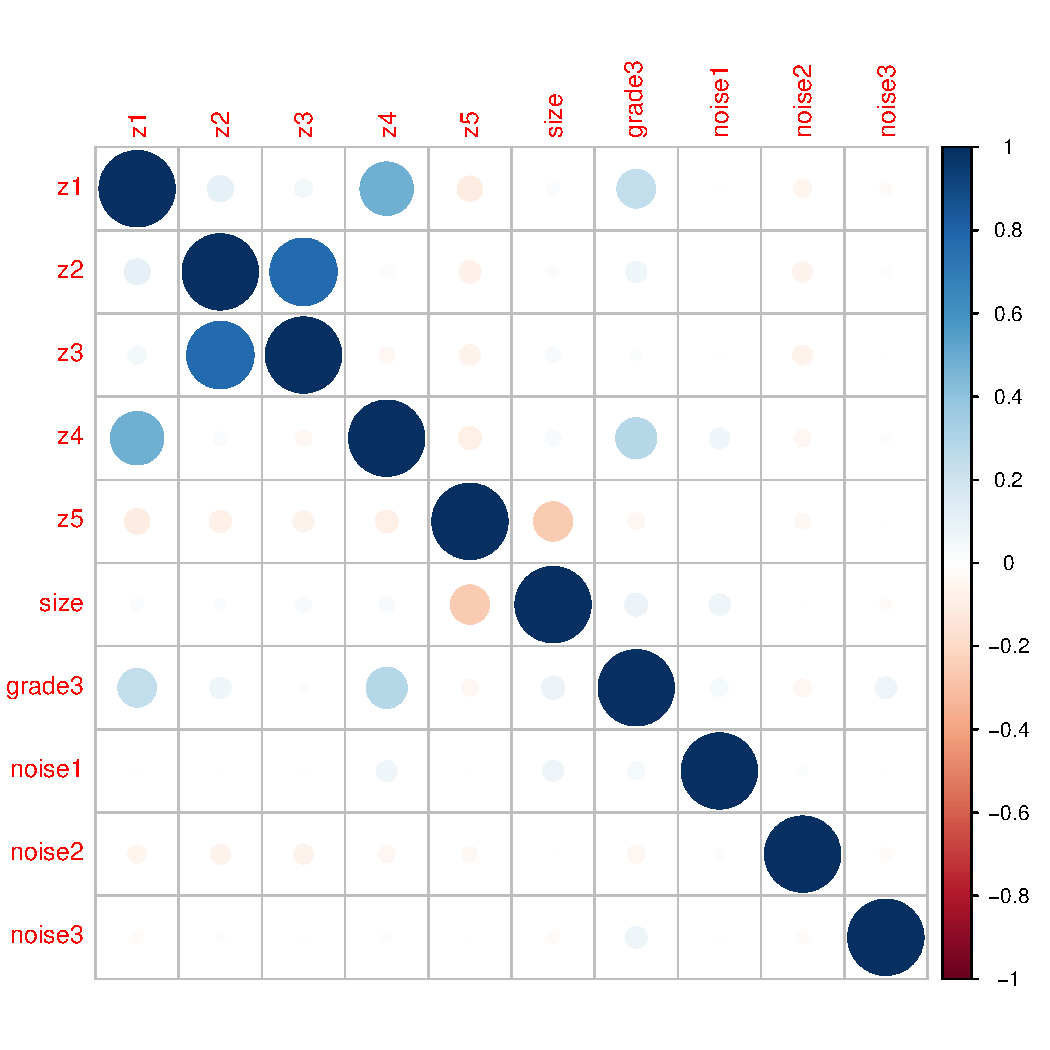
\includegraphics[width=\maxwidth]{figure/r_FSanalysis-2} 
\begin{kframe}\begin{verbatim}
## [1] "{z3}" "{z1}"
## % consistency criteria met= 1 
## SG focus= hr 
## Subgroup Consistency Minutes= 0.0227 
## Subgroup found 
## Minutes overall= 0.04415
\end{verbatim}
\begin{alltt}
\hlstd{grf.est} \hlkwb{<-} \hlkwd{grf.subg.harm.survival}\hlstd{(}\hlkwc{data} \hlstd{= x,} \hlkwc{confounders.name} \hlstd{= confounders.name,}
    \hlkwc{outcome.name} \hlstd{= outcome.name,} \hlkwc{event.name} \hlstd{= event.name,} \hlkwc{id.name} \hlstd{= id.name,} \hlkwc{treat.name} \hlstd{= treat.name,}
    \hlkwc{n.min} \hlstd{= n.min,} \hlkwc{dmin.grf} \hlstd{= dmin.grf,} \hlkwc{frac.tau} \hlstd{=} \hlnum{1}\hlstd{,} \hlkwc{details} \hlstd{=} \hlnum{TRUE}\hlstd{)}
\end{alltt}
\begin{verbatim}
## tau, maxdepth= 79.9184 2 
##   leaf.node control.mean control.size control.se treated.mean treated.size
## 1         2    -9.019098   422.000000   2.409806     9.019098   422.000000
## 2         3     1.815983   278.000000   3.062494    -1.815983   278.000000
## 3         4     7.544878   127.000000   4.298074    -7.544878   127.000000
## 4         5   -10.910407   277.000000   2.917053    10.910407   277.000000
## 5         6   -11.737772   173.000000   3.929370    11.737772   173.000000
## 6         7     6.450420   123.000000   4.577600    -6.450420   123.000000
##   treated.se       diff Nsg depth
## 1   2.409806 -18.038196 422     1
## 2   3.062494   3.631966 278     1
## 3   4.298074  15.089755 127     2
## 4   2.917053 -21.820813 277     2
## 5   3.929370 -23.475545 173     2
## 6   4.577600  12.900840 123     2
##   leaf.node control.mean control.size control.se treated.mean treated.size
## 3         4     7.544878   127.000000   4.298074    -7.544878   127.000000
##   treated.se     diff Nsg depth
## 3   4.298074 15.08976 127     2
## [1] "size <= 29" "z5 <= 0"    "z3 <= 0"   
## [1] "z5 <= 0"
\end{verbatim}
\end{kframe}
\end{knitrout}


\begin{knitrout}
\definecolor{shadecolor}{rgb}{0.969, 0.969, 0.969}\color{fgcolor}\begin{kframe}
\begin{alltt}
\hlkwd{library}\hlstd{(doParallel)}
\hlkwd{registerDoParallel}\hlstd{(parallel}\hlopt{::}\hlkwd{detectCores}\hlstd{(}\hlkwc{logical} \hlstd{=} \hlnum{FALSE}\hlstd{))}

\hlstd{cox.formula.boot} \hlkwb{<-} \hlstd{cox.formula.sim}
\hlstd{max.minutes} \hlkwb{<-} \hlnum{7}
\hlcom{# Suggest running 50, first ... to get timing estimate}

\hlstd{NB} \hlkwb{<-} \hlnum{1000}

\hlstd{df_boot_analysis} \hlkwb{<-} \hlstd{fs.est}\hlopt{$}\hlstd{df.est}

\hlstd{fitH} \hlkwb{<-} \hlkwd{get_Cox_sg}\hlstd{(}\hlkwc{df_sg} \hlstd{=} \hlkwd{subset}\hlstd{(df_boot_analysis, treat.recommend} \hlopt{==} \hlnum{0}\hlstd{),} \hlkwc{cox.formula} \hlstd{= cox.formula.boot)}
\hlstd{H_obs} \hlkwb{<-} \hlstd{fitH}\hlopt{$}\hlstd{est_obs}  \hlcom{# log(hr) scale}
\hlstd{seH_obs} \hlkwb{<-} \hlstd{fitH}\hlopt{$}\hlstd{se_obs}
\hlcom{# Hc observed estimates}
\hlstd{fitHc} \hlkwb{<-} \hlkwd{get_Cox_sg}\hlstd{(}\hlkwc{df_sg} \hlstd{=} \hlkwd{subset}\hlstd{(df_boot_analysis, treat.recommend} \hlopt{==} \hlnum{1}\hlstd{),} \hlkwc{cox.formula} \hlstd{= cox.formula.boot)}
\hlstd{Hc_obs} \hlkwb{<-} \hlstd{fitHc}\hlopt{$}\hlstd{est_obs}
\hlstd{seHc_obs} \hlkwb{<-} \hlstd{fitHc}\hlopt{$}\hlstd{se_obs}
\hlkwd{rm}\hlstd{(}\hlstr{"fitH"}\hlstd{,} \hlstr{"fitHc"}\hlstd{)}

\hlstd{Ystar_mat} \hlkwb{<-} \hlkwd{bootYstar}\hlstd{(\{}
    \hlstd{ystar} \hlkwb{<-} \hlkwd{get_Ystar}\hlstd{(boot)}
\hlstd{\},} \hlkwc{boots} \hlstd{= NB,} \hlkwc{seed} \hlstd{=} \hlnum{8316951}\hlstd{,} \hlkwc{counter} \hlstd{=} \hlstr{"boot"}\hlstd{,} \hlkwc{export} \hlstd{= fun_arg_list_boot)}
\hlcom{# Check dimension}
\hlkwa{if} \hlstd{(}\hlkwd{dim}\hlstd{(Ystar_mat)[}\hlnum{1}\hlstd{]} \hlopt{!=} \hlstd{NB} \hlopt{|} \hlkwd{dim}\hlstd{(Ystar_mat)[}\hlnum{2}\hlstd{]} \hlopt{!=} \hlkwd{nrow}\hlstd{(df_boot_analysis))} \hlkwd{stop}\hlstd{(}\hlstr{"Dimension of Ystar_mat does not match"}\hlstd{)}

\hlstd{tB.start} \hlkwb{<-} \hlkwd{proc.time}\hlstd{()[}\hlnum{3}\hlstd{]}
\hlcom{# Bootstraps}
\hlstd{resB} \hlkwb{<-} \hlkwd{bootPar}\hlstd{(\{}
    \hlstd{ans} \hlkwb{<-} \hlkwd{fsboot_forparallel}\hlstd{(boot)}
\hlstd{\},} \hlkwc{boots} \hlstd{= NB,} \hlkwc{seed} \hlstd{=} \hlnum{8316951}\hlstd{,} \hlkwc{counter} \hlstd{=} \hlstr{"boot"}\hlstd{,} \hlkwc{export} \hlstd{= fun_arg_list_boot)}
\hlstd{tB.now} \hlkwb{<-} \hlkwd{proc.time}\hlstd{()[}\hlnum{3}\hlstd{]}
\hlstd{tB.min} \hlkwb{<-} \hlstd{(tB.now} \hlopt{-} \hlstd{tB.start)}\hlopt{/}\hlnum{60}

\hlstd{doParallel}\hlopt{::}\hlkwd{stopImplicitCluster}\hlstd{()}

\hlkwd{cat}\hlstd{(}\hlstr{"Minutes for Boots"}\hlstd{,} \hlkwd{c}\hlstd{(NB, tB.min),} \hlstr{"\textbackslash{}n"}\hlstd{)}
\end{alltt}
\begin{verbatim}
## Minutes for Boots 1000 1.51255
\end{verbatim}
\begin{alltt}
\hlkwd{cat}\hlstd{(}\hlstr{"Projection per 1000"}\hlstd{,} \hlkwd{c}\hlstd{(tB.min} \hlopt{*} \hlstd{(}\hlnum{1000}\hlopt{/}\hlstd{NB)),} \hlstr{"\textbackslash{}n"}\hlstd{)}
\end{alltt}
\begin{verbatim}
## Projection per 1000 1.51255
\end{verbatim}
\begin{alltt}
\hlkwd{cat}\hlstd{(}\hlstr{"Propn bootstrap subgroups found ="}\hlstd{,} \hlkwd{c}\hlstd{(}\hlkwd{sum}\hlstd{(}\hlopt{!}\hlkwd{is.na}\hlstd{(resB}\hlopt{$}\hlstd{H_biasadj_1))}\hlopt{/}\hlstd{NB),} \hlstr{"\textbackslash{}n"}\hlstd{)}
\end{alltt}
\begin{verbatim}
## Propn bootstrap subgroups found = 0.932
\end{verbatim}
\begin{alltt}
\hlcom{# How many timmed out}
\hlkwd{cat}\hlstd{(}\hlstr{"Number timmed out="}\hlstd{,} \hlkwd{c}\hlstd{(}\hlkwd{sum}\hlstd{(}\hlkwd{is.na}\hlstd{(resB}\hlopt{$}\hlstd{H_biasadj_1)} \hlopt{&} \hlstd{resB}\hlopt{$}\hlstd{tmins_search} \hlopt{>} \hlstd{max.minutes)),}
    \hlstr{"\textbackslash{}n"}\hlstd{)}
\end{alltt}
\begin{verbatim}
## Number timmed out= 0
\end{verbatim}
\begin{alltt}
\hlstd{H_estimates} \hlkwb{<-} \hlkwd{get_dfRes}\hlstd{(}\hlkwc{Hobs} \hlstd{= H_obs,} \hlkwc{seHobs} \hlstd{= seH_obs,} \hlkwc{H1_adj} \hlstd{= resB}\hlopt{$}\hlstd{H_biasadj_2,}
    \hlkwc{ystar} \hlstd{= Ystar_mat,} \hlkwc{cov_method} \hlstd{=} \hlstr{"standard"}\hlstd{,} \hlkwc{cov_trim} \hlstd{=} \hlnum{0}\hlstd{)}
\hlstd{Hc_estimates} \hlkwb{<-} \hlkwd{get_dfRes}\hlstd{(}\hlkwc{Hobs} \hlstd{= Hc_obs,} \hlkwc{seHobs} \hlstd{= seHc_obs,} \hlkwc{H1_adj} \hlstd{= resB}\hlopt{$}\hlstd{Hc_biasadj_2,}
    \hlkwc{ystar} \hlstd{= Ystar_mat,} \hlkwc{cov_method} \hlstd{=} \hlstr{"standard"}\hlstd{,} \hlkwc{cov_trim} \hlstd{=} \hlnum{0}\hlstd{)}

\hlkwd{print}\hlstd{(H_estimates)}
\end{alltt}
\begin{verbatim}
##          H0      sdH0 H0_lower H0_upper       H1      sdH1  H1_lower H1_upper
## 1: 2.087547 0.5067638 1.297186 3.359466 1.782592 0.5326381 0.9924598 3.201775
\end{verbatim}
\begin{alltt}
\hlkwd{print}\hlstd{(Hc_estimates)}
\end{alltt}
\begin{verbatim}
##           H0       sdH0  H0_lower  H0_upper        H1      sdH1  H1_lower
## 1: 0.7448141 0.08422972 0.5967426 0.9296272 0.7489415 0.1208756 0.5458433
##    H1_upper
## 1: 1.027609
\end{verbatim}
\begin{alltt}
\hlcom{# H_estimates<-get_dfRes(Hobs=H_obs,seHobs=seH_obs,H1_adj=resB$H_biasadj_1,ystar=Ystar_mat,cov_method='standard',cov_trim=0.025)}
\hlcom{# Hc_estimates<-get_dfRes(Hobs=Hc_obs,seHobs=seHc_obs,H1_adj=resB$Hc_biasadj_1,ystar=Ystar_mat,cov_method='standard',cov_trim=0.025)}
\hlcom{# print(H_estimates) print(Hc_estimates)}


\hlstd{bootit} \hlkwb{<-} \hlkwd{list}\hlstd{(}\hlkwc{H_estimates} \hlstd{= H_estimates,} \hlkwc{Hc_estimates} \hlstd{= Hc_estimates)}
\hlstd{ans3} \hlkwb{<-} \hlkwd{fsBoot.parallel.out}\hlstd{(}\hlkwc{df} \hlstd{= df_boot_analysis,} \hlkwc{FSboots} \hlstd{= bootit,} \hlkwc{cox.formula.boot} \hlstd{= cox.formula.boot,}
    \hlkwc{sim_number} \hlstd{= sim)}
\hlstd{tall.min} \hlkwb{<-} \hlstd{(tB.now} \hlopt{-} \hlstd{t.start.all)}\hlopt{/}\hlnum{60}
\hlkwd{cat}\hlstd{(}\hlstr{"Overall minutes for analysis"}\hlstd{,} \hlkwd{c}\hlstd{(tall.min),} \hlstr{"\textbackslash{}n"}\hlstd{)}
\end{alltt}
\begin{verbatim}
## Overall minutes for analysis 1.6359
\end{verbatim}
\begin{alltt}
\hlkwd{save}\hlstd{(dgm, x, fs.est, grf.est, bootit, ans3, tall.min, resB, cox.formula.boot,} \hlkwc{file} \hlstd{=} \hlstr{"output/sim-FS4_Lasso_ex4.Rdata"}\hlstd{)}
\end{alltt}
\end{kframe}
\end{knitrout}



\begin{knitrout}
\definecolor{shadecolor}{rgb}{0.969, 0.969, 0.969}\color{fgcolor}\begin{kframe}
\begin{verbatim}
## Confounders evaluated in Forestsearch:
## [1] "noise2 <= median(noise2)" "z1"                      
## [3] "z2"                       "z3"                      
## [5] "z4"                       "z5"                      
## [7] "grade"
\end{verbatim}
\end{kframe}
\end{knitrout}





\begin{table}

\caption{\label{tab:simex_tab}\label{tab:simex} Simulated data example: Cox hazard ratio (hr) estimates for the ITT population and subgroups $H$ and $H^{c}$.
Cox model estimates are based on subgroups: H true (knowing the actual subgroup, a-priori); the estimated subgroup $\hat{H}$; and 
the boostrap ($1,000$ resamples) bias-correction to $\hat{H}$ estimates, denoted $\hat{H}_{bc}$.  Estimates for the complement $H^{c}$ are defined analogously.
The number of subjects in each population ($\#$ Subjects) and the number of subjects correctly classified ($\#$ Correct) in the true subgroups $H$ and $H^{c}$, respectively, are listed.}
\centering
\fontsize{9}{11}\selectfont
\begin{tabular}[t]{lccccc}
\toprule
  & HR Estimate & Lower & Upper & $\#$ Subjects & $\#$ Correct\\
\midrule
\addlinespace[0.3em]
\multicolumn{6}{l}{\textbf{ITT}}\\
\hspace{1em}ITT & 0.816 & 0.668 & 0.997 & 700 & .\\
\addlinespace[0.3em]
\multicolumn{6}{l}{\textbf{H subgroup estimates}}\\
\hspace{1em}$H_{oracle}$ & 2.088 & 1.297 & 3.361 & 87 & .\\
\hspace{1em}$\hat{H}$ & 2.088 & 1.297 & 3.361 & 87 & 87\\
\hspace{1em}$\hat{H}_{bc}$ & 1.783 & 0.992 & 3.203 & 87 & 87\\
\addlinespace[0.3em]
\multicolumn{6}{l}{\textbf{H-complement subgroup estimates}}\\
\hspace{1em}$H^{c}_{oracle}$ & 0.745 & 0.597 & 0.929 & 613 & .\\
\hspace{1em}$\hat{H}^{c}$ & 0.745 & 0.597 & 0.929 & 613 & 613\\
\hspace{1em}$\hat{H}^{c}_{bc}$ & 0.749 & 0.546 & 1.028 & 613 & 613\\
\bottomrule
\end{tabular}
\end{table}




\bibliographystyle{spbasic}      % basic style, author-year citations
\bibliography{../../subgroups_ref}
\end{document}
